% Document layout
\documentclass[a4paper,11pt]{article}
\usepackage[a4paper, inner=2cm , outer=2cm, top=2cm, bottom=2cm]{geometry}
\usepackage[usenames,dvipsnames]{color}
% Referencing & fonts
\usepackage[sort&compress]{natbib}
\setlength{\bibsep}{0.0pt}
\usepackage[font=small,labelfont=bf]{caption}
\usepackage[OT2,T1]{fontenc}
\usepackage{fancyvrb,courier}
\usepackage{fvextra,courier}
% Set formats for each heading level
\usepackage{sectsty}
\allsectionsfont{\usefont{OT1}{phv}{bc}{n}\selectfont}
\sectionfont{\color{MidnightBlue}} % sets colour of sections
\subsectionfont{\color{MidnightBlue}}  % sets colour of subsections
\subsubsectionfont{\color{MidnightBlue}}  % sets colour of subsections
% Other shit
\usepackage{algorithm}
\usepackage{amsfonts}
\usepackage{amsmath}
\usepackage{amssymb}
\usepackage{bbm}
\usepackage{booktabs}
\usepackage{epsfig}
\usepackage{float}
\usepackage[font=normalsize]{caption}
\usepackage{graphicx}
\usepackage{hyperref}
\usepackage{lineno}
\usepackage{mathtools}
\usepackage{sidecap}
\usepackage{sectsty}
\usepackage{verbatim}
\usepackage{wrapfig}
\usepackage{xcolor}
\usepackage{tabto}
% Declarations
\DeclarePairedDelimiter\floor{\lfloor}{\rfloor}
\DeclareSymbolFont{cyrletters}{OT2}{wncyr}{m}{n}
\DeclareMathSymbol{\Sha}{\mathalpha}{cyrletters}{"58}
\DeclareMathSymbol{\sha}{\mathalpha}{cyrletters}{"57}
% Defined commands
 \newcommand{\prgname}[1]{\textcolor{NavyBlue}{\texttt{#1}}}
 \newcommand{\linkfont}[1]{\textcolor{BurntOrange}{\textbf{#1}}}
\newcommand{\shellcmd}[1]{\\\indent\indent\texttt{\$ #1}}
\newcommand{\shellctd}[1]{\\\indent\indent\texttt{#1}}
\newcommand{\ra}[1]{\renewcommand{\arraystretch}{#1}}
\begin{document}
\begin{figure}
\centering
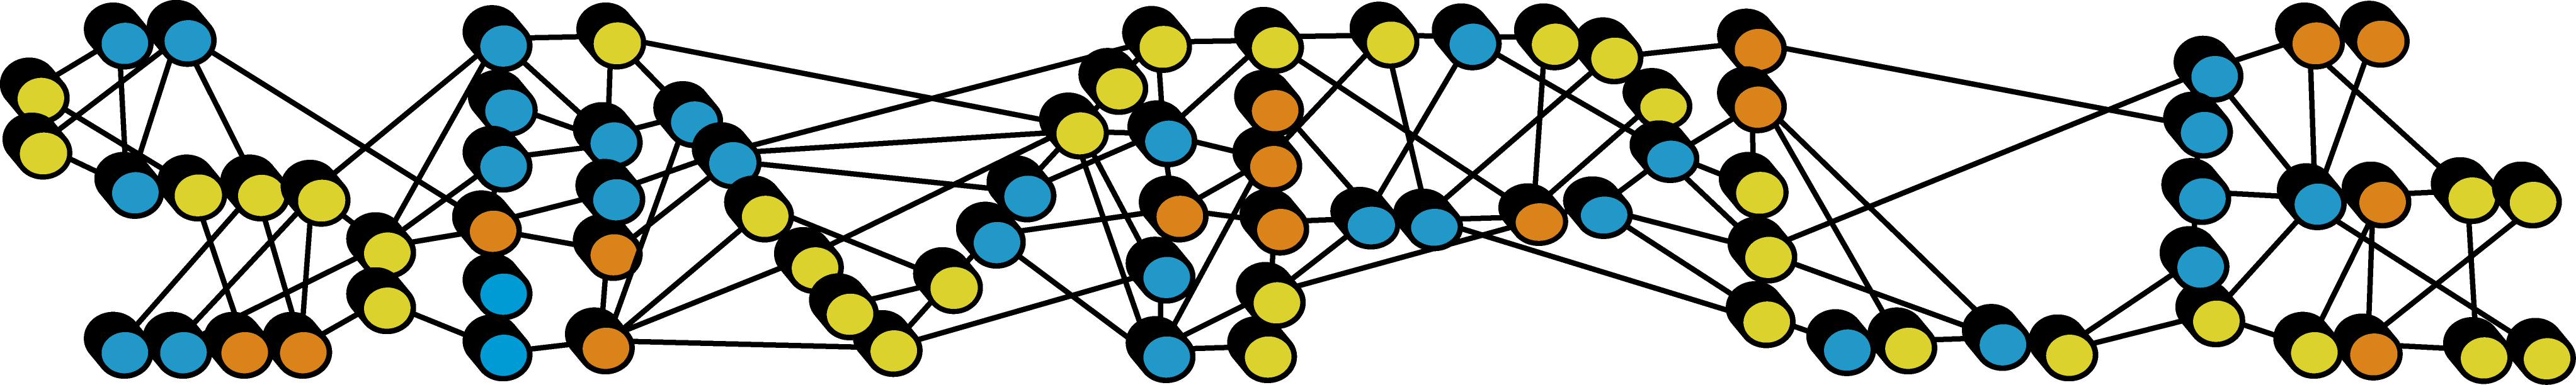
\includegraphics[keepaspectratio=true,scale=0.6]{../SIMPLE_logo/rawlogo}
%\caption{}
\end{figure}

\title{\prgname{The SIMPLE 3.0 Command-line Manual}}
\date{Jan 11, 2019}
\maketitle

\vspace{1em}
\begin{minipage}[ht]{0.50\textwidth}
\textbf{Contributors:}\\
cyril.reboul@monash.edu\\
simon.kiesewetter@monash.edu\\
chiara.machello@monash.edu\\
dominika.elmlund@monash.edu\\
hans.elmlund@monash.edu\\
\textbf{Adress:}\\
Biomedicine Discovery Institute\\
Monash University\\
3800 Clayton, VIC, Australia\\
\textbf{Webpage:}\\
www.simplecryoem.com\\
\textbf{Contact:}\\
\url{http://simplecryoem.com/contact.html}\\
dominika@simplecryoem.com\\
\end{minipage}
\vspace{20pt}

\begin{quote}
\textbf{``Keep it SIMPLE stupid''}\\(\textit{Kelly Johnson}; lead engineer at the Lockheed Skunk Works, coined the famous KISS principle stating that systems work best if they are kept simple rather than made complex. Therefore, simplicity should be a key goal in design and unnecessary complexity should be avoided.)
\end{quote}

\begin{quote}
\textbf{``Everything should be made as SIMPLE as possible, but no SIMPLEr''}\\(\textit{Albert Einstein})
\end{quote}

\begin{quote}
\textbf{``Complex theories do not work, SIMPLE algorithms do''}\\(\textit{Vladimir N. Vapnik}; author of \textit{The Nature of Statistical Learning Theory})
\end{quote}
\clearpage

\tableofcontents{}
\clearpage

\section{About SIMPLE}

\textbf{S}ingle-particle \textbf{IM}age \textbf{P}rocessing \textbf{L}inux \textbf{E}ngine (\href{www.simplecryoem.com}{\textbf{\textcolor{BurntOrange}{SIMPLE}}}) is a program package for cryo-EM image processing, covering all aspects of the single-particle analysis workflow. SIMPLE also provides tools for atomic-resolution 3D reconstruction from time-series of nanoparticles imaged in solution with graphene liquid cell TEM. The SIMPLE back-end consists of an object-oriented numerical library written in modern Fortran. In the latest SIMPLE release (version 3.0), we have revised the way that meta-data and input parameters are handled, providing a project-based execution model (described below). This model has made SIMPLE easier to use, improved output data organisation and increased performance. This document describes the command-line interface of SIMPLE and is intended for advanced users and/or developers that wish to build applications utilising the high-performance image processing algorithms in SIMPLE. <REFERENCE FOR LESS EXPERIENCED USERS>
 
SIMPLE is free software: you can redistribute it and/or modify it under the terms of the \href{http://www.gnu.org/copyleft/gpl.html}{\textbf{\textcolor{BurntOrange}{GNU General Public License}}} as published by the Free Software Foundation, either version 3 of the license, or (at your option) any later version. SIMPLE is distributed with the hope that it will be useful, but WITHOUT ANY WARRANTY; without even the implied warranty of MERCHANTABILITY or FITNESS FOR A PARTICULAR PURPOSE. See the \href{http://www.gnu.org/copyleft/gpl.html}{\textbf{\textcolor{BurntOrange}{GNU General Public License}}} for more details.

\section{Installation instructions}

\subsection{System requirements}
\begin{itemize}
	\item[--] Linux (we use Ubuntu 15.04 and above)
	\item[--] MacOSX: 10.10 and above
	\item[--] CMake 3.2 and above
	\item[--] FFTW 3.3 and above
	\item[--] GNU toolchain (gcc \& gfortran) 4.9 to 5.4
\end{itemize}

\subsection{Installation}
\noindent{}\textbf{Step 1:} Create the directory in which you are going to install SIMPLE (referred to here as \texttt{<simple\_path>})

\begin{Verbatim}[commandchars=+\[\],fontsize=\small,breaklines=true]
mkdir <simple_path>
\end{Verbatim}

\noindent{}\textbf{Step 2:} Unzip the SIMPLE 3.0 tar ball in this directory (assuming you have downloaded the tar ball in the \texttt{<downloads>} directory)

\begin{Verbatim}[commandchars=+\[\],fontsize=\small,breaklines=true]
mv <downloads>/SIMPLE3.0.tgz <simple path>
cd <simple path>
tar -xzf SIMPLE3.0.tgz
\end{Verbatim}

\noindent{}\textbf{Step 3:} Create a directory for the build

\begin{Verbatim}[commandchars=+\[\],fontsize=\small,breaklines=true]
cd simple3.0
mkdir build
cd build
\end{Verbatim}

\noindent{}\textbf{Step 4:} Compile and install SIMPLE 3.0

\begin{Verbatim}[commandchars=+\[\],fontsize=\small,breaklines=true]
cmake ../
make -j install
\end{Verbatim}

\noindent{}This will install SIMPLE in the \texttt{'build'} directory, clean out all unnecessary
files and will finish with the following message (a reminder for step 5 below):

\begin{Verbatim}[commandchars=+\[\],fontsize=\small,breaklines=true]
Installation complete.
==========================================================================
Please ensure the following variables are set properly in add2.*rc file:
    SIMPLE_EMAIL SIMPLE_QSYS SIMPLE_PATH SIMPLE_SOURCE_PATH
To use SIMPLE, append the relevant add2.* to your HOME shell rc file:
  bash$ cat add2.bashrc >> ~/.bashrc
  tcsh$ cat add2.tcshrc >> ~/.tcshrc
==========================================================================
For minimal installation to work correctly add:
<your src path>/Simple-release/build/bin and
<your src path>/Simple-release/build/scripts
to your PATH environment variable.
==========================================================================
\end{Verbatim}

\noindent{}When the build and installation directories are the same (default) and you are
happy with the install, you may want to clean compilation-generated and
unnecessary files using \texttt{distclean}.

\begin{Verbatim}[commandchars=+\[\],fontsize=\small,breaklines=true]
make distclean
\end{Verbatim}

\noindent{}If you wish to provide an alternative installation directory, substitute step 4 with

\begin{Verbatim}[commandchars=+\[\],fontsize=\small,breaklines=true]
cmake -DCMAKE_INSTALL_PREFIX=<alternative directory> ../
make -j install
\end{Verbatim}

\noindent{}Step 4 assumes that gcc/gfortran and FFTW are installed in fairly standard directories on your machine. In case you have a 
more exotic setup you can provide the paths pointing to your custom gcc/gfortran \& FFTW by substituting step 4 with

\begin{Verbatim}[commandchars=+\[\],fontsize=\small,breaklines=true]
FC=<gcc/gfortran path> FFTW_DIR=<FFTW path> cmake ../
make -j install
\end{Verbatim}

\noindent{}For instance, on MacOS:
\begin{itemize}
	\item[--] Macports users may use: FC=/opt/local/bin/gfortran FFTW\_DIR=/opt/local;
	\item[--] Fink users: FC=/sw/bin/gfortran FFTW\_DIR=/sw/; and
	\item[--] Homebrew users: FC=/usr/local/bin/gfortran FFTW\_DIR=/usr/local/
\end{itemize}

\noindent{}\\\textbf{Step 5:} Set the environment variables.

\noindent{}\\To run SIMPLE, the bin and scripts paths need to be in the \texttt{PATH} environment
variable. The \texttt{SIMPLE\_PATH} environment variable must also be defined. The 
shell scripts \texttt{add2.bashrc} and \texttt{add2.tcshrc} containing the necessary
instructions were generated during the build step. For immediate use for running and testing, execute

\begin{Verbatim}[commandchars=+\[\],fontsize=\small,breaklines=true]
source add2.bashrc
\end{Verbatim}

\noindent{}or, for TCSH/CSH users:

\begin{Verbatim}[commandchars=+\[\],fontsize=\small,breaklines=true]
source add2.tcshrc
\end{Verbatim}

\noindent{}For permanent installation \texttt{BASH} users should add the contents of \texttt{add2.bashrc} to your \texttt{<HOME>/.bashrc}

\begin{Verbatim}[commandchars=+\[\],fontsize=\small,breaklines=true]
cat add2.bashrc >> ~/.bashrc
\end{Verbatim}

\noindent{}or for TCSH/CSH users:

\begin{Verbatim}[commandchars=+\[\],fontsize=\small,breaklines=true]
cat add2.tcshrc >> ~/.tcshrc
\end{Verbatim}

\subsection{Testing the build}

\noindent{}To ensure that SIMPLE has been correctly installed, we recommend running the application \texttt{simple\_test\_install}. It will test the most 
important components in the SIMPLE library  (those used by prime2D and  prime3D). Execute

\begin{Verbatim}[commandchars=+\[\],fontsize=\small,breaklines=true]
simple_test_install 
\end{Verbatim}

\noindent{}The program will create its own folder \texttt{SIMPLE\_TEST\_INSTALL*date*} where temporary files and information about each 
test are stored. Upon succesful completion you should see

\begin{Verbatim}[commandchars=+\[\],fontsize=\small,breaklines=true]
 **** SIMPLE_TEST_INSTALL NORMAL STOP ****
\end{Verbatim}

\noindent{}\texttt{simple\_test\_install} can be executed anywhere. After execution, the folder created can be safely removed. If any of the individual 
tests fail an error message will be displayed. If you detect an error, please carefully check the SIMPLE and FFTW installations 
and the gfortran version. If you still have issues, please file a help ticket on the webpage.

\subsection{Installation/configuration on a Linux cluster}

Installation on a Linux cluster is essentially the same as on a Linux workstation with the exception that the appropriate modules need to be loaded before installation and execution. On a typical SLURM cluster
\begin{Verbatim}[commandchars=+\[\],fontsize=\small,breaklines=true]
module load fftw/3.3.4-gcc
module load gcc/4.9.1
\end{Verbatim}
The instructions for how to execute SIMPLE in distributed environments (clusters or workstations with more than one CPU socket) are described below \label{distr}.

\subsection{What is new in SIMPLE release 3.0?}
The number of changes we have made to the suite compared to the previously released version (2.5) are too many to list here. If you have experience with previous SIMPLE releases, please have a quick browse through the manual. We promise you will catch-up quickly. Most (but not all) of the algorithms implemented in SIMPLE have been published (REFS). If you want to understand the theory, we recommend you read the papers. This document exclusively describes the command-line driven SIMPLE user interface and basic knowledge about EM and single-particle analysis is assumed. 

\subsubsection{SIMPLE program naming convention}
The first big change you will notice is that all program names have changed to plain English descriptions of their functionality.  For example, \prgname{PRIME2D} that does simultaneous 2D alignment and clustering in a reference-free manner is now called \prgname{cluster2D}, the workflow for \textit{ab initio} 3D reconstruction from class averages is called \prgname{initial\_3Dmodel}, the 3D refinement application is called \prgname{refine3D} and the heterogeneity analysis tool is called \prgname{cluster3D}. In SIMPLE, we distinguish between \textit{distributed workflows} (executed with \texttt{simple\_distr\_exec}) and \textit{programs} (executed with \texttt{simple\_exec}). Programs perform smaller tasks (subjected exclusively to OpenMP-thread-based parallelisation), whereas distributed workflows are major image processing steps that typically require a multi-core workstation or a computer cluster. Finally, there is a third executable \texttt{simple\_private\_exec} that is used internally by SIMPLE, by the SIMPLE developers and by very advanced users that want to test experimental aspects of SIMPLE or use functionality to support building GUI applications on top of SIMPLE.

\subsubsection{SIMPLE input parameter categorisation}
Another noticeable change is they way the command-line instructions are provided when you execute a SIMPLE program or distributed workflow. For example, this is what is written in the terminal when executing \texttt{simple\_distr\_exec prg=refine3D}
\begin{Verbatim}[commandchars=+\[\],fontsize=\small,breaklines=true]
+underline[USAGE]
+textit[bash-3.2$ simple_distr_exec prg=refine3D key1=val1 key2=val2 ...]
Required input parameters in +textbf[bold] (ensure terminal support)
+underline[IMAGE INPUT/OUTPUT]
vol1 = Reference volume; input volume e.g. vol.mrc
+underline[SEARCH CONTROLS]
+textbf[pgrp         = Point-group symmetry; point-group(cn|dn|t|o|i){c1}]
center       = Center reference volume(s); (yes|no){yes}
continue     = Continue previous refinement; (yes|no){no}
frac         = Fraction of particles to include; fraction of particles(0.1-0.9){1.0}
maxits       = Max iterations; Max # iterations
neigh        = Neighbourhood refinement; (yes|no){no}
nnn          = Number of nearest neighbours; # projection neighbours{10% of search space}
nrestarts    = Number of restarts; # restarts{1}
nspace       = Number of projection directions; # projections
nstates      = Number of states; # states to reconstruct
objfun       = Objective function; (cc|ccres|euclid){cc}
refine       = Refinement mode; (snhc|single|multi|greedy_single|cont_single|greedy_multi|cluster|clustersym){single}
sigma2_fudge = Sigma2-fudge factor; {100.}
trs          = Maximum translational shift; max shift per iteration in pixels{5}
update_frac  = Fractional update per iteration; update this fraction per iter(0.1-0.5){1.0}
+underline[FILTER CONTROLS]
cenlp      = Centering low-pass limit; centering low-pass limit in Angstroms{30}
eo         = Gold-standard FSC for filtering and resolution estimation; (yes|no){no}
hp         = High-pass limit; high-pass limit in Angstroms
lp         = Static low-pass limit; low-pass limit in Angstroms
lplim_crit = Low-pass limit FSC criterion; low-pass FSC criterion(0.143-0.5){0.3}
lpstop     = Low-pass limit for frequency limited refinement; low-pass limit in Angstroms
shellw     = B-factor weighted reconstruction; (yes|no){no}
+underline[MASK CONTROLS]
+textbf[msk      = Mask radius; mask radius in pixels]
focusmsk = Mask radius in focused refinement; focused mask radius in pixels
inner    = Inner mask radius; inner mask radius in pixels
mskfile  = Input mask file; e.g. automask.mrc from postprocess
width    = Falloff of inner mask; # pixels cosine edge{10}
+underline[COMPUTER CONTROLS]
+textbf[nparts = Number of parts; divide job into # parts]
+textbf[nthr   = Number of threads per part, give 0 if unsure; # shared-memory CPU threads]
\end{Verbatim}

\noindent{}The number of input parameters can be daunting and to simplify the representation we have divided them into the following categories.

\begin{itemize}
    \item[--] \textbf{IMAGE INPUT/OUTPUT} consists of MRC format stacks or volumes.
    \item[--] \textbf{PARAMETER INPUT/OUTPUT} are parameters associated with the inputted images.
    \item[--] \textbf{ALTERNATIVE INPUTS} is for programs that accept alternative inputs: volume or stack, for example.
    \item[--] \textbf{SEARCH CONTROLS} are parameters that control optimisation.
    \item[--] \textbf{FILTER CONTROLS} are parameters that control Fourier filtering options.
    \item[--] \textbf{MASK CONTROLS} are parameters that control real-space masking options.
    \item[--] \textbf{COMPUTER CONTROLS} are parameters that specifies how to utilise the computing environment.
\end{itemize}

\noindent{}The required command-line parameters are printed in \textbf{bold}. Hence, the execution of  \texttt{simple\_distr\_exec prg=refine3D} could be as trivial as

\begin{Verbatim}[commandchars=+\[\],fontsize=\small,breaklines=true]
simple_distr_exec prg=refine3D pgrp=c1 msk=120 nparts=4 nthr=8
\end{Verbatim}

\noindent{}We have encapsulated all the details of the SIMPLE user interface in an abstract data type. A JSON description of the SIMPLE user interface can be obtained through 

\begin{Verbatim}[commandchars=+\[\],fontsize=\small,breaklines=true]
simple_private_exec prg=write_ui_json
\end{Verbatim}

\noindent{}This produces the file \texttt{simple\_user\_interface.json} describing all distributed workflows and programs in SIMPLE. This may be useful for building GUI applications on top of the SIMPLE back-end.

\subsubsection{SIMPLE project execution model}

The final major change that affects SIMPLE usage is the project-based execution model that encapsulates all meta-data in a single file and provides a complete and reversible history of the SIMPLE project. This is best illustrated by example. Below, we provide the commands executed for reconstructing HCN (EMPIAR-10081) to 3.4 A resolution.

\begin{Verbatim}[commandchars=+\[\],fontsize=\small,breaklines=true]
simple_exec prg=new_project projname=hcn_test
\end{Verbatim}

\noindent{}This creates the project, represented by a directory created in the current working directory called \texttt{hcn\_test} and in that directory a binary file called \texttt{hcn\_test.simple} that will be filled up with meta-data as the project progresses. Next, we change directory to the project directory and import some data.

\begin{Verbatim}[commandchars=+\[\],fontsize=\small,breaklines=true]
cd hcn_test
simple_exec prg=import_particles cs=2.7 ctf=yes fraca=0.1 kv=300 smpd=1.3 stk=/media/hael/LongTermStorage/EM-data/HCN/hcn_shiny.mrc deftab=/media/hael/LongTermStorage/EM-data/HCN/deftab.txt
\end{Verbatim}

\noindent{}This imports an MRC stack with associated CTF parameters to the project. If you list the content of the project directory you will see that the directory \texttt{1\_import\_particles} was created, containing a \texttt{hcn\_test.simple} file. What happened here? First, the import program created its execution directory, then made a copy of the project file and in that copy it imported the stack file path and CTF parameter information. The next command is for running a 2D analysis

\begin{Verbatim}[commandchars=+\[\],fontsize=\small,breaklines=true]
nohup simple_distr_exec prg=cluster2D ncls=200 msk=65 nparts=4 nthr=32 > CLS2D &
\end{Verbatim}

\noindent{}By default, SIMPLE looks in the project directory and picks the project file from the execution directory with the highest number as a starting point for the next process. In this example, the 2D analysis picks the project file from the \texttt{1\_import\_particles}. Sometimes you may want to start from another project file and selecting the highest numbered one is not desired. Therefore, the possibility to provide a project file on the command line is given.
\begin{Verbatim}[commandchars=+\[\],fontsize=\small,breaklines=true]
projfile=X_execution_dir/project_file.simple
\end{Verbatim}

\noindent{}If desired, it is also possible to turn off the execution directory generation and run the process straight in the current working directory. This is done by giving
\begin{Verbatim}[commandchars=+\[\],fontsize=\small,breaklines=true]
mkdir=no
\end{Verbatim}
\noindent{}on the command line. In a realistic situation, you would have used \prgname{cleanup2D} in replacement of \prgname{cluster2D} to remove junk and identify good particles. If you have a GUI running on top of the SIMPLE back-end you would then like to report any selections made in the GUI to the project file. Below, we describe how to do this. This data set was already cleaned with RELION, so we proceed using all class averages for initial 3D model production.

\begin{Verbatim}[commandchars=+\[\],fontsize=\small,breaklines=true]
nohup simple_distr_exec prg=initial_3Dmodel pgrp=c4 hp=60 msk=65 nparts=4 nthr=32 > INI3D &
\end{Verbatim}

\noindent{}Finally, we execute the refinement command

\begin{Verbatim}[commandchars=+\[\],fontsize=\small,breaklines=true]
nohup simple_distr_exec prg=refine3D pgrp=c4 frac=0.9 maxits=15 trs=5 update_frac=0.2 eo=yes hp=60 msk=65 nparts=4 nthr=32 > REFINE3D &
\end{Verbatim}

\noindent{}The final and intermittent results are neatly organised in directories in the project directory

\begin{Verbatim}[commandchars=+\[\],fontsize=\small,breaklines=true]
ls
1_import_particles  3_initial_3Dmodel  CLS2D            INI3D     stack_parts
2_cluster2D         4_refine3D         hcn_test.simple  REFINE3D
\end{Verbatim}

\noindent{}and it is possible to go back to any point in the project history to re-run a job with different parameters or try a different algorithm for the task. Now, let's look closer at the project file.

\subsubsection{Structure, interrogation and manipulation of the binary project file}
In SIMPLE v3.0 we have implemented an abstract data type called sp\_project that manages all meta-data generated throughout a single-particle analysis project. The multi-segment binary project file is simply a mirror of this data type on disk. Segments 1-10 are reserved  for simple program outputs, orientations and files. Currently implemented segments are

\begin{enumerate}
    \item micrographs
    \item per-micrograph stacks
    \item per-particle 2D orientations
    \item per-cluster 2D orientations
    \item per-cluster 3D orientations
    \item per-particle 3D orientations
    \item critical project outputs
\end{enumerate}

\noindent{}Segments 11-20 are reserved for project info, job management etc. Currently implemented segments are

\begin{enumerate}
   \setcounter{enumi}{10}
    \item project information
    \item command lines of processes executed
    \item computing environment specification
\end{enumerate}

\noindent{}All of these segments utilise the SIMPLE orientation container object for data storage and we therefore refer to the different segment types as ``oritype'' with shorthand descriptors

\begin{enumerate}
    \item micrographs, \tab{}\texttt{oritype = \textbf{mic}}
    \item per-micrograph stacks, \tab{}\texttt{oritype = \textbf{stk}}
    \item per-particle 2D orientations, \tab{}\texttt{oritype = \textbf{ptcl2D}}
    \item per-cluster 2D orientations, \tab{}\texttt{oritype = \textbf{cls2D}}
    \item per-cluster 3D orientations, \tab{}\texttt{oritype = \textbf{cls3D}}
    \item per-particle 3D orientations, \tab{}\texttt{oritype = \textbf{ptcl3D}}
    \item critical project outputs,\tab{}\texttt{oritype = \textbf{out}}
\end{enumerate}

\begin{enumerate}
   \setcounter{enumi}{10}
    \item project information, \tab{}\texttt{oritype = \textbf{projinfo}}
    \item command lines of processes executed, \tab{}\texttt{oritype = \textbf{jobproc}}
    \item computing environment specification, \tab{}\texttt{oritype = \textbf{compenv}}
\end{enumerate}

\noindent{}The first method of choice for interrogating the project file is

\begin{Verbatim}[commandchars=+\[\],fontsize=\small,breaklines=true]
simple_exec prg=print_project_info
\end{Verbatim}

\noindent{}Going back to out HCN example, we cd to the \texttt{hcn\_test/4\_refine3D} execution directory and execute \texttt{simple\_exec prg=print\_project\_info}. This produces the output
\begin{Verbatim}[commandchars=+\[\],fontsize=\small,breaklines=true]
+underline[+textbf[SEGMENT 02 of type: stk]]
+textit[4 record(s) of stack (extracted particles) info, one per stack of particles]
+textbf[first record:] stk=../stack_parts/stack_part1.mrc stkkind=split imgkind=ptcl phaseplate=no ctf=yes box=256.000000 nptcls=13968.0000 fromp=1.00000000 top=13968.0000 smpd=1.29999995 kv=300.000000 cs=2.70000005 fraca=0.100000001 state=1.00000000
+underline[+textbf[SEGMENT 03 of type: ptcl2D]]
+textit[55870 record(s) of 2D information generated by cluster2D, one per particle]
+textbf[first record:] kv=300.000000 cs=2.70000005 fraca=0.100000001 dfx=4.13821840 dfy=4.34016752 angast=11.1103058 state=1.00000000 eo=0.00000000 stkind=1.00000000 x=-1.87167823 y=-3.53704500 updatecnt=18.0000000 w=1.00000000 bfac_rec=0.00000000 lp=7.16521692 e3=280.975616 inpl=37.0000000 class=128.000000 corr=0.342293173 specscore=0.198325723 bfac=514.059692 dist_inpl=0.00000000 mi_class=1.00000000 frac=100.000000 e1=0.00000000 e2=0.00000000
+underline[+textbf[SEGMENT 04 of type: cls2D]]
+textit[200 record(s) of data generated by cluster2D, one per 2D cluster]
+textbf[first record:] class=1.00000000 pop=254.000000 res=7.53409100 corr=0.340087920 w=1.00000000 specscore=0.242327988 state=1.00000000
+underline[+textbf[SEGMENT 05 of type: cls3D]]
+textit[200 record(s) of 3D information for class averages, one per class]
+textbf[first record:] dfx=0.00000000 dfy=0.00000000 angast=0.00000000 state=1.00000000 x=-1.16237819 y=-1.83902657 e1=12.5358458 e2=158.906311 e3=305.373138 proj=2409.00000 w=1.00000000 bfac=23.9044113 mi_proj=1.00000000 mi_state=1.00000000 dist=6.78878576E-02 dist_inpl=0.00000000 frac=100.000000 corr=0.943886340 specscore=0.941106677 inpl=1.00000000 spread=0.986059248 shwmean=0.169503510 shwstdev=7.38897547E-02 npeaks=11.0000000 updatecnt=23.0000000 ow=0.173722118 class=1.00000000 lp=10.1947365 stkind=1.00000000
+underline[+textbf[SEGMENT 06 of type: ptcl3D]]
+textit[55870 record(s) of 3D information, one per particle]
+textbf[first record:] kv=300.000000 cs=2.70000005 fraca=0.100000001 dfx=4.13821840 dfy=4.34016752 angast=11.1103058 state=1.00000000 eo=0.00000000 stkind=1.00000000 x=-2.17266393 y=-3.59118795 w=0.00000000 bfac_rec=0.00000000 lp=3.52181816 e3=300.895508 inpl=2.00000000 class=128.000000 corr=0.106535442 specscore=6.47827759E-02 bfac=143.173950 dist_inpl=0.895474195 mi_class=1.00000000 frac=100.000000 e1=1.58313191 e2=92.8490295 proj=1295.00000 updatecnt=3.00000000 dist=2.52782822 ow=2.80490033E-02 spread=3.31418705 shwmean=0.493733585 shwstdev=0.237732679 npeaks=74.0000000 mi_proj=0.857142866
+underline[+textbf[SEGMENT 07 of type: out]]
+textit[6 record(s) of crtitical project outputs: class averages, 3D volumes, FSC/FRC files etc.]
+textbf[first record:] frcs=../2_cluster2D/frcs.bin imgkind=frc2D
+underline[+textbf[SEGMENT 11 of type: projinfo]]
+textit[1 record(s) of information about the project, project name etc.]
+textbf[first record:] projname=hcn_test projfile=hcn_test.simple cwd=/Processing/HCN/hcn_test
+underline[+textbf[SEGMENT 12 of type: jobproc]]
+textit[4 record(s) of all command-lines executed throughout the project]
+textbf[first record:] prg=import_particles ctf=yes stk=/media/hael/LongTermStorage/EM-data/HCN/hcn_shiny.mrc deftab=/media/hael/LongTermStorage/EM-data/HCN/deftab.txt mkdir=yes projfile=/Processing/HCN/hcn_test/1_import_particles/hcn_test.simple projname=hcn_test exec_dir=1_import_particles date=20190104.0 time=161342.797 cs=2.70000005 fraca=0.100000001 kv=300.000000 smpd=1.29999995
+underline[+textbf[SEGMENT 13 of type: compenv]]
+textit[1 record(s) of computing environment specifications, queue system, memory per job etc.]
+textbf[first record:] simple_path=/home/hael/src/SIMPLE3.0/build qsys_name=local user_email=my.name@uni.edu job_name=simple_hcn_test time_per_image=100.000000 job_memory_per_task=16000.0000
\end{Verbatim}

\noindent{}You notice that what happened in the HCN workflow is directly reflected in the project file structure. The \prgname{cluster2D} analysis split the imported stack into four parts (one per partition used), which is why the \texttt{\textbf{stk}} segment contains 4 records. The first record of the segment is also printed and we see that the first record of the \texttt{\textbf{stk}} segment contains the filename in addition to a number of parameters associated with the stack file, represented by key-value entries. Next, the \prgname{cluster2D} analysis filled-in the \texttt{\textbf{ptcl2D}} segment with 55870 records (one per particle) and the \texttt{\textbf{cls2D}} segment with 200 records (one per class). Subsequently, the \prgname{initial\_3Dmodel} workflow provided 200 records in the \texttt{\textbf{cls3D}} segment, describing class average orientations. Finally, the  \prgname{refine3D} workflow provided 55870 records of 3D orientations and various other statistics (one per particle) in the \prgname{ptcl3D} segment. There are 7 records of critical project outputs in the \texttt{\textbf{out}} segment (SEGMENT 07) and to inspect them closer we use the following command

\begin{Verbatim}[commandchars=+\[\],fontsize=\small,breaklines=true]
simple_exec prg=print_project_field oritype=out
\end{Verbatim}

\noindent{}This produces the output

\begin{Verbatim}[commandchars=+\[\],fontsize=\small,breaklines=true]
frcs=../2_cluster2D/frcs.bin imgkind=frc2D
stk=../2_cluster2D/cavgs_iter018.mrc stkkind=single imgkind=cavg ctf=no box=256.000000 nptcls=200.000000 fromp=1.00000000 top=200.000000 smpd=1.29999995
vol=../3_initial_3Dmodel/rec_final.mrc imgkind=vol_cavg box=256.000000 smpd=1.29999995 state=1.00000000
fsc=../4_refine3D/fsc_state01.bin imgkind=fsc state=1.00000000 box=256.000000
vol=../4_refine3D/aniso_optlp_state01.mrc imgkind=vol_filt box=256.000000 smpd=1.29999995 state=1.00000000
vol=../4_refine3D/recvol_state01_iter015.mrc imgkind=vol box=256.000000 smpd=1.29999995 state=1.00000000
\end{Verbatim}

\noindent{}\prgname{cluster2D} provided two critical outputs: a file of Fourier Ring Correlations (\texttt{frcs}) and a stack of class averages (\texttt{stk}). \prgname{initial\_3Dmodel} provided one volume output. Finally, \prgname{refine3D} provided three outputs: Fourier Shell Correlations (\texttt{fsc}) and two volumes. 



% Volta phase-plate support


\section{File formats}

\subsection{Image file formats}
SIMPLE supports SPIDER (\texttt{*.spi}) and MRC (\texttt{*.mrc}) formats for image stacks and volumes. The MRC file handling classes are shared with the the FREALIX program for helical reconstruction \citep{Rohou:2014aa}. RELION \citep{Scheres:2012aa} uses the convention that MRC stacks have the suffix \texttt{*.mrcs} and volumes the suffix \texttt{*.mrc}. This is to overcome the annoyance that it is not possible to tell from an MRC file header whether a MRC file is a volume or a stack. With SIMPLE you can select to use either the \texttt{*.mrcs} or \texttt{*.mrc} suffix for stacks. The way that we keep track of whether a file is a volume or stack is via the command line key value. The key-value pairs \texttt{vol1=rec.mrc} and \texttt{vol2=rec2.mrc} refer to volumes whereas the key-value pairs \texttt{stk=ptcls.mrc} and \texttt{stk2=ptcls2.mrc} refer to stacks.

\subsection{SIMPLE parameter file format}
The SIMPLE text-files used for parameter input/output use a \texttt{key=value} syntax of the form
\begin{Verbatim}[commandchars=+\[\],fontsize=\small,breaklines=true]
e1=80. e2=100. e3=5.5 x=1.23 y=4.25 dfx=2.56 dfy=2.54 angast=30.5 state=1
\end{Verbatim}
to represent per-particle information. Internally, the orientation information is stored in a dynamic hash data structure, which gives the file format high flexibility. Therefore, writing conversion scripts to allow interchange of parameters between SIMPLE and other packages is easy. SIMPLE uses the same conventions as FREALIGN \citep{Grigorieff:2007aa} to represent orientations and CTF parameters. The CTF parameterisation obtained by CTFFIND \citep{Mindell:2003aa} can be directly plugged into SIMPLE, for example by creating a file \texttt{deftab.txt}, looking like
\begin{Verbatim}[commandchars=+\[\],fontsize=\small,breaklines=true]
dfx=2.56 dfy=2.76 angast=30.5
dfx=3.50 dfy=3.33 angast=60.0
dfx=1.98 dfy=2.02 angast=120.5
...
\end{Verbatim}
It is also possible to import data using plain text files, as described below.

\subsection{Parameter File Conversions}
The \texttt{SIMPLE/scripts} folder contains perl-scripts (\texttt{convert\_frealign2simple.pl}) and\\ (\texttt{convert\_relion2simple.pl}) to convert FREALIGN and RELION parameter files, respectively, file to a SIMPLE parameter file. This is easy, since these software packages internally use the \href{http://spider.wadsworth.org/spider_doc/spider/docs/euler.html}{\textbf{\textcolor{BurntOrange}{Spider Euler angle convention}}}. Other packages may use other conventions. There's also a \texttt{relion2emanbox.pl} script for converting box files obtained with RELION to the EMAN \texttt{*.box} format used by SIMPLE.



\section{SIMPLE usage}

\subsection{SIMPLE help tools}
In attempt to reduce the dependency on the manual, we have packaged a lot of the documentation in the software itself. For example
\begin{Verbatim}[commandchars=+\[\],fontsize=\small,breaklines=true]
simple_exec prg=list
center
cluster_cavgs
convert
ctfops
export_starproject
extract
filter
fsc
info_image
info_stktab
import_boxes
...
\end{Verbatim}
lists all programs executed with \texttt{simple\_exec} (shared-memory parallelisation) and
\begin{Verbatim}[commandchars=+\[\],fontsize=\small,breaklines=true]
simple_distr_exec prg=list
cleanup2D
cluster2D
cluster2D_stream
cluster3D
cluster3D_refine
ctf_estimate
gen_pspecs_and_thumbs
initial_3Dmodel
make_cavgs
motion_correct
motion_correct_tomo
pick
pick_extract_stream
preprocess
preprocess_stream
reconstruct3D
refine3D
refine3D_init
scale_project
tseries_track
\end{Verbatim}
lists all distributed workflows executed with \texttt{simple\_distr\_exec}. If you don't quite remember which program you are looking for but remember that it was called \texttt{cluster} something, you could execute
\begin{Verbatim}[commandchars=+\[\],fontsize=\small,breaklines=true]
simple_distr_exec prg=list | grep cluster
cluster2D
cluster2D_stream
cluster3D
cluster3D_refine
\end{Verbatim}
If you want a description for a particular program, for example \prgname{cluster2D}, execute
\begin{Verbatim}[commandchars=+\[\],fontsize=\small,breaklines=true]
simple_distr_exec prg=cluster2D describe=yes
is a distributed workflow implementing a reference-free 2D alignment/clustering algorithm adopted from the prime3D probabilistic ab initio 3D reconstruction algorithm
\end{Verbatim}
To obtain a description of the what command line options are available, execute
\begin{Verbatim}[commandchars=+\[\],fontsize=\small,breaklines=true]
simple_distr_exec prg=cluster2D
\end{Verbatim}

\subsection{Categorisation and description of SIMPLE distributed workflows}

\subsubsection{PRE-PROCESSING WORKFLOWS}
\begin{itemize}
\item[--] \prgname{preprocess} is a distributed workflow that executes \prgname{motion\_correct}, \prgname{ctf\_estimate} and \prgname{pick} in sequence
\item[--] \prgname{preprocess\_stream} is a distributed workflow that executes \prgname{motion\_correct}, \prgname{ctf\_estimate} and \prgname{pick} in streaming mode as the microscope collects the data
\item[--] \prgname{motion\_correct} is a distributed workflow for motion correction of movies based on the same principal strategy as Grigorieff's program. There are two important differences: automatic weighting of the frames using a correlation-based M-estimator and continuous optimisation of the shift parameters. If dose\_rate and exp\_time are given the individual frames will be low-pass filtered accordingly (dose-weighting strategy). If scale is given, the movie will be Fourier cropped according to the down-scaling factor (for super-resolution movies). If nframesgrp is given the frames will be pre-averaged in the given chunk size (Falcon 3 movies). If fromf/tof are given, a contiguous subset of frames will be averaged without any dose-weighting applied
\item[--] \prgname{gen\_pspecs\_and\_thumbs} is a distributed workflow for generating power spectra and thumbnails for imported integrated movies
\item[--] \prgname{motion\_correct\_tomo} is a distributed workflow for motion correction of movies based on the same principal strategy as Grigorieff's program. There are two important differences: automatic weighting of the frames using a correlation-based M-estimator and continuous optimisation of the shift parameters. If dose\_rate and exp\_time are given the individual frames will be low-pass filtered accordingly (dose-weighting strategy). The exp\_doc document should contain per line \texttt{exp\_time=X} and \texttt{dose\_rate=Y}. It is assumed that the input list of movies (one per tilt) are ordered temporally. This is necessary for correct dose-weighting of tomographic tilt series. If scale is given, the movie will be Fourier cropped according to the down-scaling factor (for super-resolution movies). If \texttt{nframesgrp} is given the frames will be pre-averaged in the given chunk size (Falcon 3 movies)
\item[--] \prgname{ctf\_estimate} is a distributed SIMPLE workflow for CTF parameter fitting
\item[--] \prgname{pick} is a distributed workflow for template-based particle picking
\item[--] \prgname{pick\_extract\_stream} is a distributed workflow for template-based particle picking and extraction in streaming mode
\end{itemize}

\subsubsection{CLUSTER2D WORKFLOWS}
\begin{itemize}
\item[--] \prgname{make\_cavgs} is a distributed workflow for generating class averages or initial random references for \prgname{cluster2D} execution
\item[--] \prgname{cleanup2D} is a distributed workflow implementing a reference-free 2D alignment/clustering algorithm suitable for the first pass of cleanup after picking
\item[--] \prgname{cluster2D} is a distributed workflow implementing a reference-free 2D alignment/clustering algorithm adopted from the prime3D probabilistic ab initio 3D reconstruction algorithm
\item[--] \prgname{cluster2D\_stream} is a distributed workflow implementing \prgname{cluster2D} in streaming mode
\end{itemize}

\subsubsection{AB INITIO 3D RECONSTRUCTION WORKFLOW}
\begin{itemize}
\item[--] \prgname{initial\_3Dmodel} is a distributed workflow for generating an initial 3D model from class averages obtained with \prgname{cluster2D}
\end{itemize}

\subsubsection{REFINE3D WORKFLOWS}
\begin{itemize}
\item[--] \prgname{refine3D\_init} is a distributed workflow for generating a random initial 3D model for initialisation of \prgname{refine3D}
\item[--] \prgname{refine3D} is a distributed workflow for 3D refinement based on probabilistic projection matching
\item[--] \prgname{reconstruct3D} is a distributed workflow for reconstructing volumes from MRC and SPIDER stacks, given input orientations and state assignments. The algorithm is based on direct Fourier inversion with a Kaiser-Bessel (KB) interpolation kernel
\end{itemize}

\subsubsection{CLUSTER3D WORKFLOWS}
\begin{itemize}
\item[--] \prgname{cluster3D} is a distributed workflow for heterogeneity analysis by 3D clustering
\item[--] \prgname{cluster3D\_refine} is a distributed workflow based on probabilistic projection matching for refinement of 3D heterogeneity analysis by \prgname{cluster3D}
\end{itemize}

\subsubsection{TIME-SERIES WORKFLOWS}
\begin{itemize}
\item[--] \prgname{tseries\_track} is a distributed workflow for particle tracking in time-series data
\end{itemize}

\subsubsection{MISCELLANEOUS WORKFLOWS}
\begin{itemize}
\item[--] \prgname{scale\_project} is a distributed workflow for re-scaling MRC \& SPIDER stacks part of project specification
\end{itemize}

\subsection{Categorisation and description of SIMPLE programs}

\subsubsection{PROJECT MANAGEMENT PROGRAMS}
\begin{itemize}
\item[--] \prgname{new\_project} is a program for creating a new project. SIMPLE3.0 relies on a monolithic project file for controlling execution on distributed and shared-memory systems and for unified meta-data management. This program creates a directory named projname and a file projname.simple inside that directory that contains all information about the project as well as all meta data generated by the different SIMPLE programs. This file is mirrored by an abstract data type in the back-end, which manages the parameters and meta-data I/O required for execution of SIMPLE
\item[--] \prgname{update\_project} is a program for updating an existing project: changing the name/user\_email/ computer controls
\item[--] \prgname{print\_project\_info} is a program prints information about a *.simple project file
\item[--] \prgname{print\_project\_field} is a program for printing an orientation field in the project data structure (segment in *.simple project file)
\item[--] \prgname{import\_movies} is a program for importing DDD movies to the project. The movies can be located in any read-only location accessible to the project. If the movies contain only a single frame, they will be interpreted as motion-corrected and integrated. Box files (in EMAN1.9 format) can be imported along with the movies
\item[--] \prgname{import\_boxes} is a program for importing EMAN1.9 box coordinates to the project. The *box (text) files should be listed in boxtab
\item[--] \prgname{import\_particles} is a program for importing extracted particle images to the project
\item[--] \prgname{import\_cavgs} is a program for importing class averages movies to the project
\item[--] \prgname{subset\_project} is a program that generates a random subset of an existing project
\item[--] \prgname{export\_starproject} is a program for exporting a SIMPLE project as a STAR-formatted EM project
\item[--] \prgname{import\_starproject} is a program for importing STAR-formatted EM project files to the current SIMPLE project and saving as a SIMPLE project
\item[--] \prgname{report\_selection} is a program for reporting external (GUI) selections to the SIMPLE project
\end{itemize}

\subsubsection{SINGLE-PARTICLE WORKFLOW PROGRAMS}
\begin{itemize}
\item[--] \prgname{extract} is a program for extracting particle images from integrated movies
\item[--] \prgname{reextract} is a program for re-extracting particle images from integrated movies based on determined 2D/3D shifts
\item[--] \prgname{cluster\_cavgs} is a program for analyzing class averages with affinity propagation, in order to get a better understanding of the view distribution. The balance flag is used to apply a balancing restraint (on the class population). Adjust balance until you are satisfied with the shape of the histogram
\item[--] \prgname{symaxis\_search} is a program for searching for the principal symmetry axis of a volume reconstructed in C1. The rotational transformation is applied to the oritype field in the project and the project file is updated. If you are unsure about the point-group, use the \prgname{symmetry\_test} program instead
\item[--] \prgname{symmetry\_test} is a program that implements a statistical test for point-group symmetry. Input is a volume reconstructed without symmetry (c1) and output is the most likely point-group symmetry
\item[--] \prgname{postprocess} is a program for map post-processing. Use program volops to estimate the B-factor with the Guinier plot
\end{itemize}

\subsubsection{IMAGE PROCESSING PROGRAMS}
\begin{itemize}
\item[--] \prgname{mask} is a program for masking of 2D images and volumes. If you want to mask your images with a spherical mask with a soft  falloff, set msk to the radius in pixels
\item[--] \prgname{fsc} is a program for calculating the FSC between the two input volumes
\item[--] \prgname{local\_resolution} is a program for estimating local resolution based on neighbourhood correlation analysis in e/o maps
\item[--] \prgname{local\_resolution2D} is a program for estimating local resolution based on neighbourhood correlation analysis in e/o cavgs
\item[--] \prgname{center} is a program for centering a volume and mapping the shift parameters back to the particle images
\item[--] \prgname{reproject} is a program for re-projecting a volume using Fourier interpolation. Input is a SPIDER or MRC volume. Output is a stack of projection images of the same format as the inputted volume. Projections are generated by extracting central sections from the Fourier volume and back transforming the 2D FTs. nspace controls the number of projection directions. The  oritab parameter allows you to input the orientations that you wish to have your volume projected in. pgrp controls the point-group symmetry c (rotational), d (dihedral), t (tetrahedral), o (octahedral) or i (icosahedral). The point-group symmetry is used to restrict the set of projections to within the asymmetric unit. neg inverts the contrast of the projections
\item[--] \prgname{volops} is a program that provides standard single-particle image processing routines for MRC or SPIDER volumes
\item[--] \prgname{convert} is a program for converting between SPIDER and MRC formats
\item[--] \prgname{ctfops} is a program for applying CTF to stacked images
\item[--] \prgname{filter} is a program for filtering stack/volume
\item[--] \prgname{normalize} is a program for normalization of MRC or SPIDER stacks and volumes
\item[--] \prgname{scale} is a program for re-scaling, clipping and padding MRC \& SPIDER stacks and volumes
\item[--] \prgname{stack} is a program for stacking individual images (list) or multiple stacks into one
\item[--] \prgname{stackops} is a program that provides standard single-particle image processing routines for MRC or SPIDER stacks. To extract a particular state, give \texttt{oritab} and set \texttt{state}. To select the fraction of best particles, give \texttt{oritab} and set frac. State and frac options can be combined. To apply noise, give the desired signal-to-noise ratio via snr. To calculate the autocorrelation function, set acf=yes. To extract a contiguous subset of images from the stack, set fromp and top. To extract a number of particle images at random, set nran to the desired number. With avg=yes the global average of the stack is calculated. If nframesgrp is set to some integer number >1, averages with chunk sizes of nframesgrp are produced, which may be useful for analysis of dose-fractionated image series. neg inverts the contrast of the images
\item[--] \prgname{shift} is a program for shifting a stack according to origin shifts in oritab
\end{itemize}

\subsubsection{ORIENTATION PROCESSING PROGRAMS}
\begin{itemize}
\item[--] \prgname{make\_oris} is a program for making SIMPLE orientation files. Random Euler angles and random origin shifts are generated. If ndiscrete is set to an integer number > 0, the orientations produced are randomly sampled from the set of ndiscrete quasi-even projection directions, and the in-plane parameters are assigned randomly. If even is set to yes, then all nptcls orientations are assigned quasi-even projection directions and  random in-plane parameters. If nstates is set to some integer number > 0, then states are assigned randomly
\item[--] \prgname{orisops} is a program for modifying SIMPLE orientation/parameter files. If errify=yes, uniform random angular errors, and uniform origin shift errors,  and uniform random defocus errors are introduced. If nstates > 1 then random states are assigned. If mirr=2d, then the Euler angles in oritab are mirrored according to the relation e1=e1, e2=180+e2, e3=-e3. If mirr=3d, then the Euler angles in oritab are mirrored according to the relation R=M(M*R), where R is the rotation matrix calculated from the Euler angle triplet and M is a 3D reflection matrix. If e1, e2, or e3 is inputted, the orientations are rotated correspondingly. If you input state, only the orientations assigned to state state are rotated. If mul is defined, the origin shifts are multiplied with mul. If zero=yes, then the shifts are zeroed
\item[--] \prgname{oristats} is a program for analyzing SIMPLE orientation/parameter files. If two orientation tables (oritab and oritab2) are inputted, statistics of the distances between the orientations in the two documents are provided
\item[--] \prgname{vizoris} is a program for extracting projection directions from orientations for visualization in UCSF Chimera
\end{itemize}

\subsubsection{PRINT INFO PROGRAMS}
\begin{itemize}
\item[--] \prgname{info\_image}
\item[--] \prgname{info\_stktab}
\item[--] \prgname{print\_fsc}
\item[--] \prgname{print\_frcs}
\item[--] \prgname{print\_magic\_boxes}
\end{itemize}

\subsubsection{SIMULATOR PROGRAMS}
\begin{itemize}
\item[--] \prgname{simulate\_noise}
\item[--] \prgname{simulate\_particles}
\item[--] \prgname{simulate\_movie}
\item[--] \prgname{simulate\_subtomogram}
\end{itemize}

\subsubsection{SYSTEM INTERACTION PROGRAMS}
\begin{itemize}
\item[--] \prgname{mkdir}
\end{itemize}

\subsection{Execution of SIMPLE}
SIMPLE is executed primarily via \texttt{simple\_distr\_exec} that implements higher level workflows intended for distributed execution on workstations and clusters using a hybrid parallelisation model (distributed \textit{and} shared memory). SIMPLE can also be executed via \texttt{simple\_exec}, which implements all individual SIMPLE programs and runs in shared-memory parallelisation mode. Please, beware that the high-level workflows (\prgname{prime2D} and \prgname{ini3D\_from\_cavgs}, for example) can \textit{only} be executed via the distributed execution route. In cluster environments using a job scheduler (PBS, SLURM and SGE are supported by SIMPLE) the file \texttt{simple\_distr\_config.env} in the current working directory controls the execution.
\begin{Verbatim}[commandchars=+\[\],fontsize=\small,breaklines=true]
bash-3.2$ cat simple_distr_config.env 
# CONFIGURATION FILE FOR DISTRIBUTED SIMPLE EXECUTION

# ABSOLUTE PATH TO SIMPLE ROOT DIRECTORY
simple_path           = /scratch/m3earlyadopters/simple/simple/

# ESTIMATED TIME PER IMAGE (IN SECONDS)
time_per_image        = 600

# USER DETAILS
user_account          = el85 
user_email            = hans.elmlund@monash.edu
user_project          = 

# QSYS DETAILS (qsys_name=<local|slurm|pbs>)
qsys_name             = slurm
qsys_partition        = m3a
qsys_qos              =
qsys_reservation      = simple

# JOB DETAILS
job_ntasks            = 1
job_memory_per_task   = 48000
job_name              = taf-dna-part2
job_ntasks_per_socket = 1
\end{Verbatim}
This file is auto-generated on workstations, but it needs to be edited by the user in cluster environments. If you need help configuring distributed SIMPLE execution, please file a help ticket on the webpage. The two most important parameters for distributed execution is the number of partitions \texttt{nparts} and the number of shared-memory CPU threads \texttt{nthr}. A rule of thumb for good performance on multi-socket workstations is to minimise the number of parts and maximising the number of threads subject to never having fewer parts than sockets. The shared memory parallelisation does not benefit from the use of a larger number of threads than the number of logical threads available on a socket. To check the number of processors on a linux system, execute \texttt{nproc} in the terminal. Consider a heterogeneous cluster with N nodes, two CPU sockets per node and six CPUs per socket.
\begin{SCfigure}[][h]
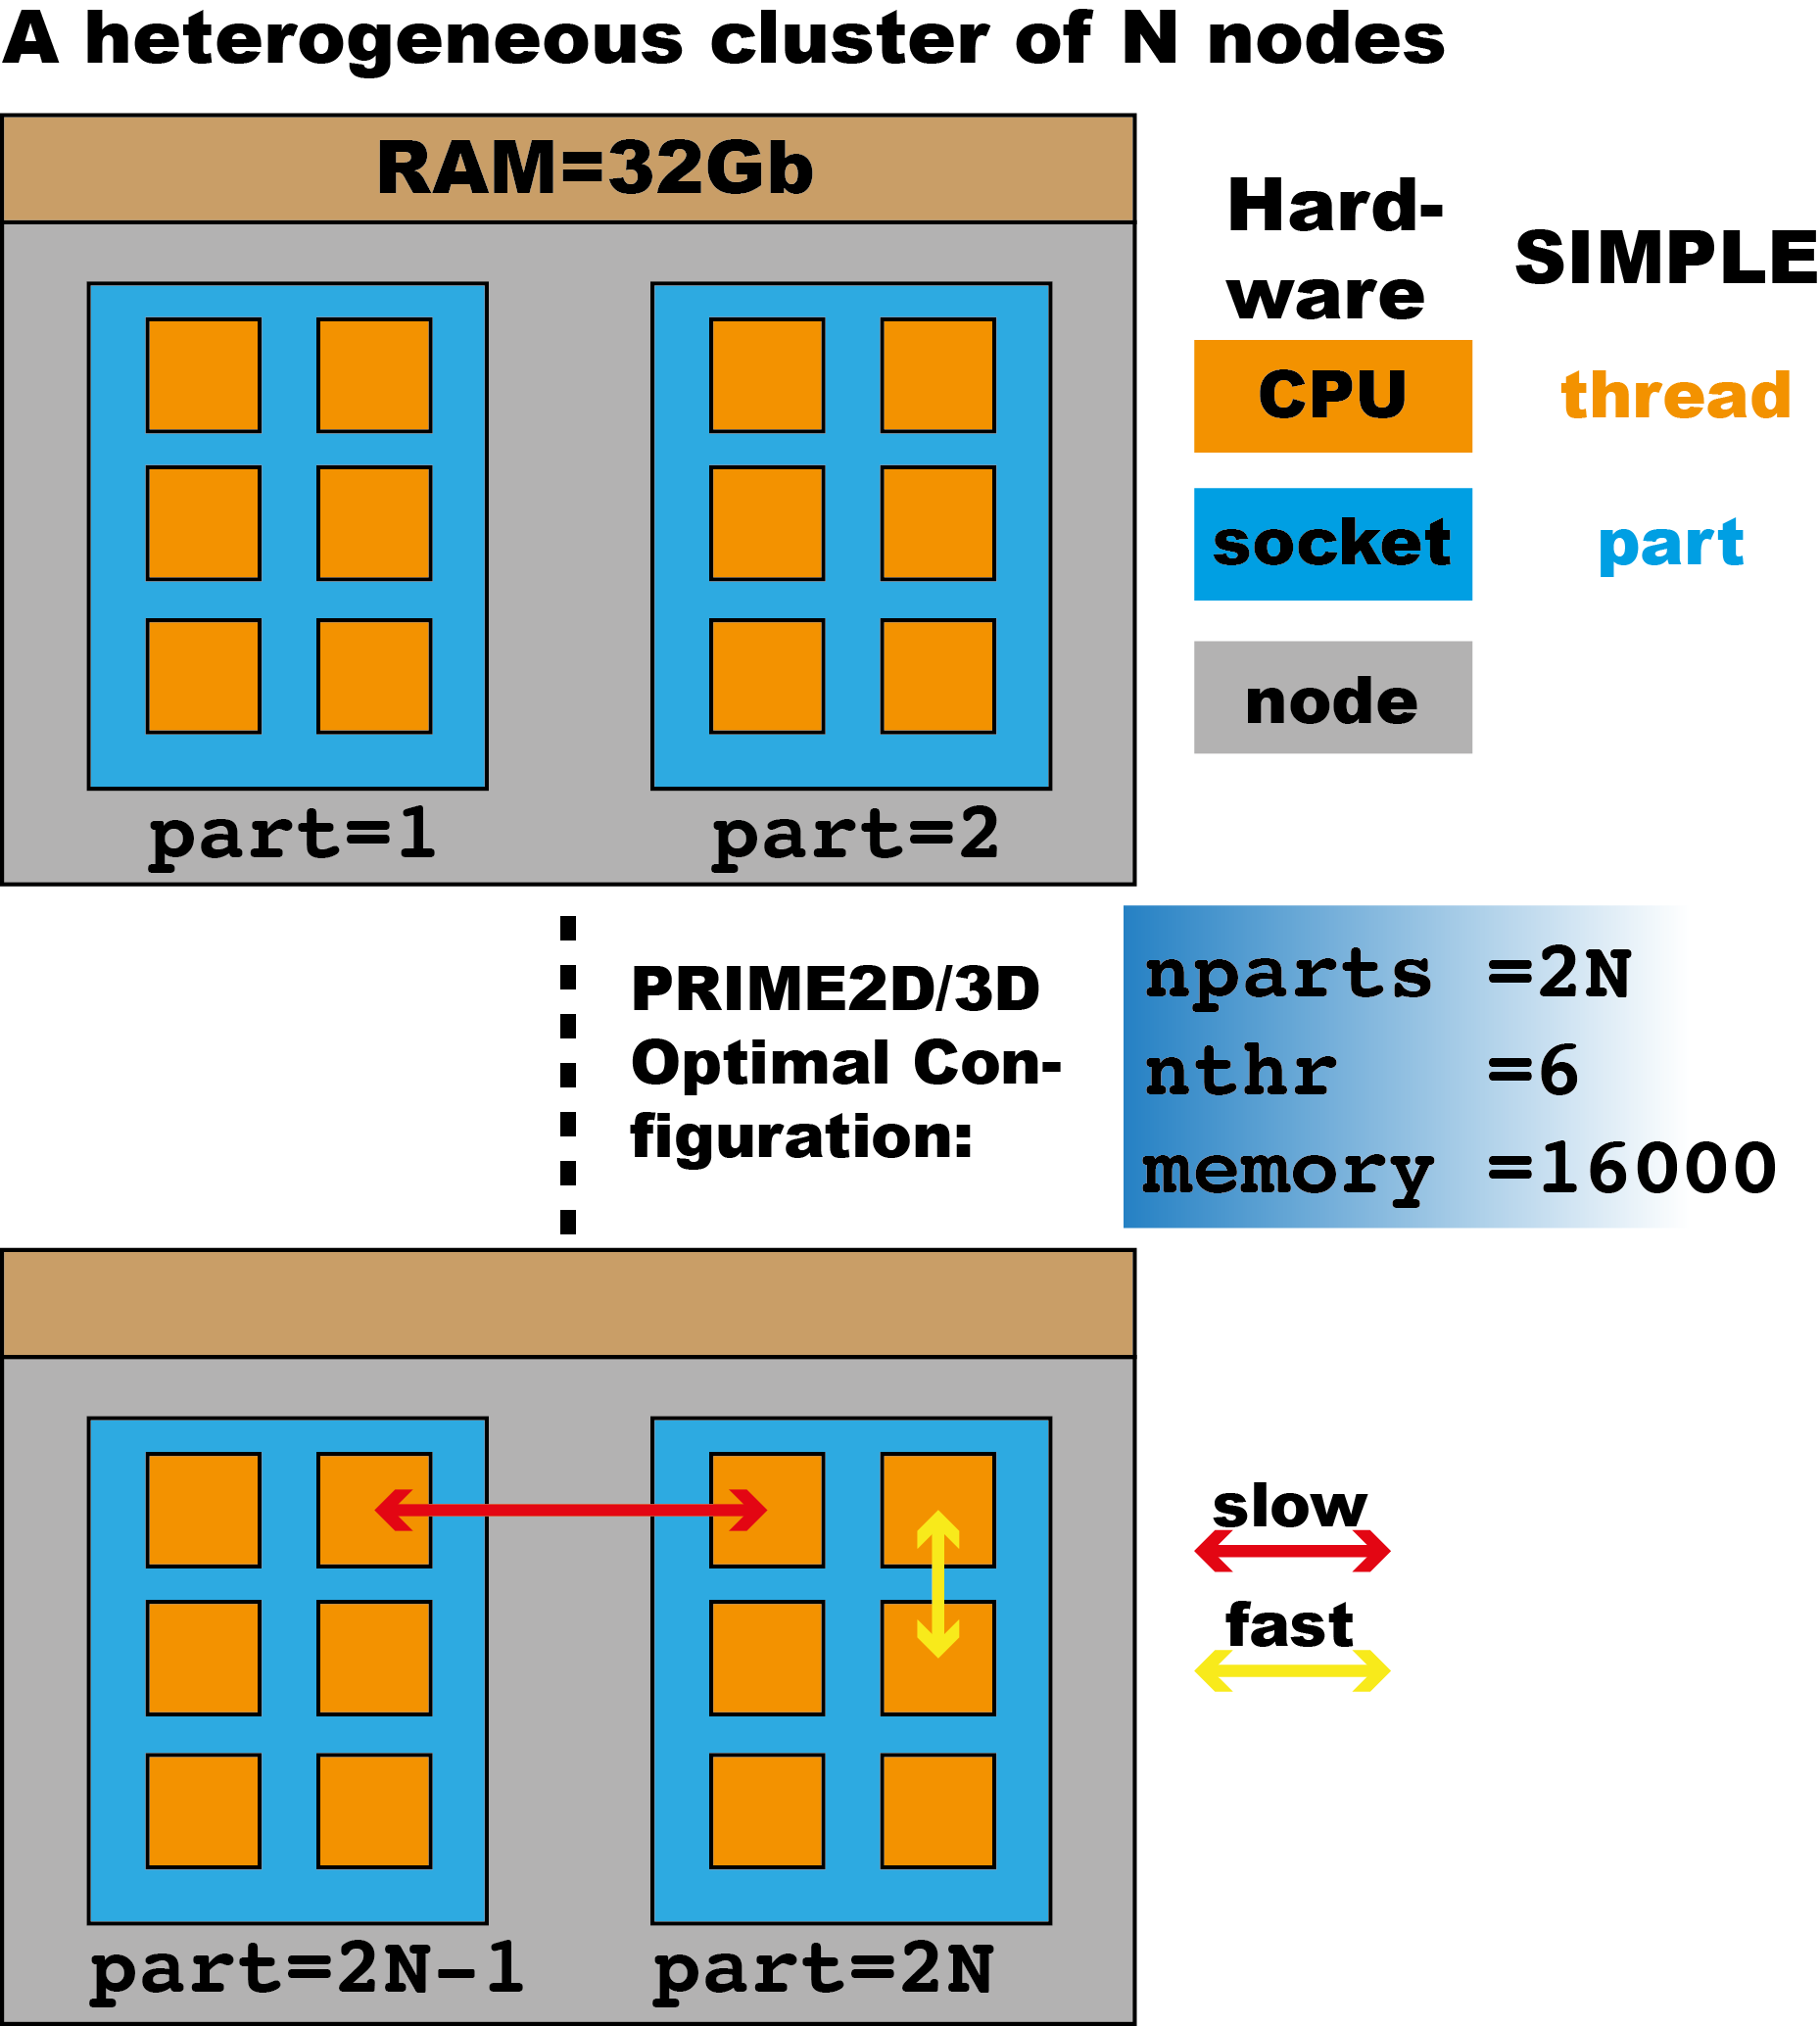
\includegraphics[keepaspectratio=true,scale=0.6]{../CPUtopo/cputopo}
\caption{\textbf{Configuration of the parallel PRIME-2D/3D execution on a heterogeneous cluster.} We here represent the nodes in  a heterogeneous cluster by two sockets with six CPUs each and 32Gb RAM/node. The best performance of PRIME--2D/3D is going to be obtained by partitioning  the jobs into \texttt{npart=2N} partitions, where \texttt{N} is the number of nodes. Each partition will then execute six threads \texttt{nthr=6} and these six threads will get access to half the RAM on the node (\texttt{memory=16000}) because we have two sockets per node that need to share the RAM between them}
\end{SCfigure}
If you are unsure how to configure your SIMPLE execution please file a help ticket.

We normally let \prgname{simple\_distr\_exec} run in the background on the login node of our cluster. An example of how to distribute \prgname{prime2D} using ten nodes is provided below.
\begin{Verbatim}[commandchars=+\[\],fontsize=\small,breaklines=true]
nohup simple_distr_exec prg=prime2D stk=ptcls.mrc smpd=1.77 msk=100
ncls=600 nthr=8 nparts=10 >> PRIME2DOUT &
\end{Verbatim}
Another option available on clusters that use the SLURM scheduler is to use the \texttt{srun} command for \prgname{simple\_distr\_exec} via
\begin{Verbatim}[commandchars=+\[\],fontsize=\small,breaklines=true]
srun --ntasks=1 --ntasks-per-socket=1 --cpus-per-task=1 --mem=32000 
--time=2-0:0:0 --output=PRIME2DOUT.%j --error=PRIME2DERR.%j
simple_distr_exec prg=prime2D stk=ptcls.mrc smpd=1.77 msk=100
ncls=600 nthr=8 nparts=10 &
\end{Verbatim}
However, beta testers have reported that srun job sometimes dies with no warning, possibly because of the low tolerance for network errors. A more robust route may be to use \texttt{sbatch} as follows
\begin{Verbatim}[commandchars=+\[\],fontsize=\small,breaklines=true]
sbatch -p MYCLUSTER --wrap="simple_distr_exec prg=prime2D stk=ptcls.mrc 
smpd=1.77 msk=100 ncls=600 nthr=8 nparts=10 >> PRIME2DOUT"
\end{Verbatim}
where the \texttt{--wrap} flag automatically generates a bash script for the given command.

\subsection{From Movies to Near-atomic Resolution Map}
These steps describe a typical SIMPLE workflow.
\begin{enumerate}
\item DDD (Direct Detector Device) movie alignment and frame-weighting using SIMPLE program \prgname{unblur}, executed with \texttt{simple\_distr\_exec}
\item CTF parameter identification with the SIMPLE program \prgname{ctffind}, wrapping CTFFIND4 \citep{rohou2015ctffind4}, executed with \texttt{simple\_distr\_exec}
\item Particle identification using EMAN2 \citep{Tang:2007aa} to generate \texttt{*.box} files
\item Particle extraction with SIMPLE program \prgname{extract}, executed with \texttt{simple\_exec}
\item 2D analysis using the SIMPLE \prgname{prime2D} distributed workflow, executed with \texttt{simple\_distr\_exec}
\item \textit{Ab initio} 3D reconstruction from class averages using the SIMPLE \prgname{ini3D\_from\_cavgs} distributed workflow, executed with \texttt{simple\_distr\_exec}
\item Mapping of class average selection and 3D class orientations to the particles using SIMPLE program \prgname{map2ptcls}, executed with \texttt{simple\_exec}
\item Reconstruction of a 3D map from the individual particle images with SIMPLE program \prgname{recvol}, executed with \texttt{simple\_distr\_exec}
\item Map refinement will be part of release 3.0
\end{enumerate}
For descriptions for how to execute the individual steps, please refer to the documentation of each program (below).

\subsection{Workflows for Analysis of Time-series data of Nanoparticles Spinning in Solution}
In addition to providing algorithms for analysis of electron microscopic projection images of biological molecules, SIMPLE also provides support for time-series analysis of nanoparticles spinning in solution.
\subsubsection{Time-series Pre-processing}
\begin{enumerate}
\item Convert the time-series from \texttt{*.dm4} format to the \texttt{*.mrc} format using the \prgname{dm42mrc.pl} script. This script assumes that you have \texttt{EMAN2} installed on your system.
\item Use the \prgname{tseries\_extract} program to generate overlapping windows of frames in the time series. We recommend a window size of 5. This program is executed via \texttt{simple\_exec prg=tseries\_extract}. The \texttt{frameavg} flag controls the size of the time-window.
\item Correct for stage drift and global beam-induced motion by processing the \texttt{*tseries\_frames*} stacks with \prgname{unblur}. It is important that you set \texttt{lpstart=5} and \texttt{lpstop=3} in addition to the required input parameters.
\item Use \texttt{EMAN1.9} or \texttt{EMAN2} to identify, in the first motion corrected frame, the particles that you want to track throughout the time-series. Write out a \texttt{*.box} file with the particle coordinates.
\item Use the \texttt{*.box} file created in the previous step in conjunction with the motion-corrected frames as input to the program \prgname{tseries\_track} to generate individual stacks of images representing the windowed nanoparticles as a function of time from the first to the last frame. Please execute \prgname{tseries\_track} using the \texttt{simple\_distr\_exec} binary. This will run the tracker in parallel mode with one CPU allocated per particle. The \texttt{ncunit} parameter controls the number of CPUs being used and this number cannot be larger than the number of particles to track in parallel.
Once the pre-processing workflow has been finalised, the problem becomes a standard single-particle reconstruction problem (one per particle stack). However, as SIMPLE was originally designed for biological single-particle EM image processing, there are a few parameter tuning strategies to consider (described below).
\end{enumerate}

\def\bibfont{\footnotesize}
\bibliographystyle{cell}
\bibliography{Prime2bibfile}

\end{document}
